To further understand how coordination facts work, we present other programs that
take advantage of them.

\subsection{Belief Propagation}

Randomized and approximation algorithms can obtain significant benefits from
coordination directives because although the final program results will not be
exact, they follow important statistical properties and can be computed faster.
An examples of such programs is PageRank~\cite{Lubachevsky:1986:CAA:4904.4801}
and Loopy Belief Propagation~\cite{Gonzalez+al:aistats09paraml}, which is the
focus of this section.

Loopy Belief Propagation (LBP) is an approximate inference algorithm used in
graphical models with cycles~\cite{Murphy99loopybelief}. In its essence, LBP is
a sum-product message passing algorithm where nodes exchange messages with their
immediate neighbors and apply some computations to the messages received.

LBP is an algorithm that maps very well to the graph-based model of LM. The
original algorithm computes the belief of all nodes for several iterations with
synchronization between iterations. However, it is possible to avoid the
synchronization step, if we take advantage of the fact that LBP will converge
even when using an asynchronous approach. So, instead of computing the belief
iteratively, we keep track of all messages sent/received (and overwrite them
when we receive a new one) and recompute the belief asynchronously.
Figure~\ref{fig:coordination:bp} shows the communication patterns for our
application and Fig.~\ref{code:coordination:bp} presents the LM code for the
implementation.

\begin{figure}[h]
   \begin{center}
      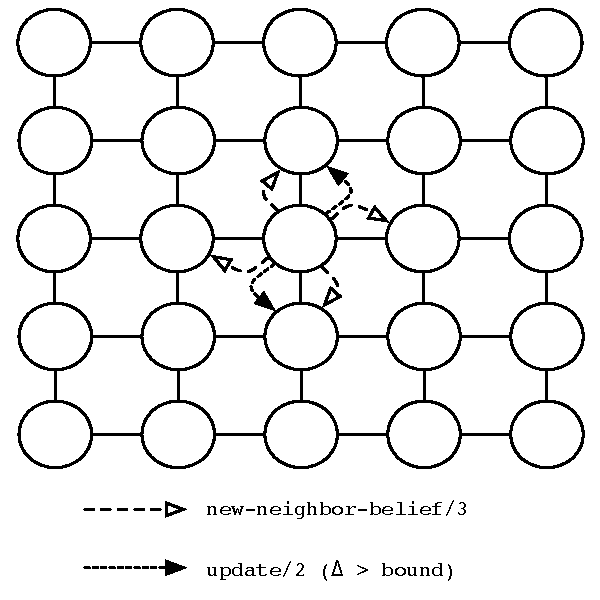
\includegraphics[width=0.3\textwidth]{figures/bp/bp.pdf}
   \end{center}
\caption{LBP: communication patterns}
\label{fig:coordination:bp}
\end{figure}

\begin{figure}[h!]
\begin{Verbatim}[numbers=left, fontsize=\codesize, commandchars=\*\{\}]
neighbor-belief(A, B, Belief),*label{line:coord:bp_first1}
new-neighbor-belief(A, B, NewBelief)
   -o neighbor-belief(A, B, NewBelief).*label{line:coord:bp_first2}

check-residual(A, Residual, B),*label{line:coord:bp_check1}
Residual > bound
   -o update(B).
check-residual(A, _, _) -o 1.*label{line:coord:bp_check2}

// update belief to be sent to one neighbor*label{line:coord:bp_iterate1}
update-messages(A, NewBelief),
!edge(A, B),
neighbor-belief-old(A, B, OldIn),
sent-neighbor-belief(A, B, OldOut),
Cavity = normalize(divide(NewBelief, OldIn)),
Convolved = normalize(convolve(global-potential, Cavity)),
OutMessage = damp(Convolved, OldOut, damping)
   -o Residual = residual(OutMessage, OldOut),
      check-residual(A, Residual, B),
      update-messages(A, NewBelief),
      new-neighbor-belief(B, A, OutMessage),
      sent-neighbor-belief(A, B, OutMessage).*label{line:coord:bp_iterate2}

update-messages(A, NewBelief) -o 1.*label{line:coord:bp_iterate_final}

// if we have two update functions, just run one of them*label{line:coord:bp_last1}
update(A), update(A) -o update(A).*label{line:coord:bp_update}

// make a copy of neighbors beliefs in order to add them up*label{line:coord:bp_update1}
update(A),
!potential(A, Potential),
belief(A, MyBelief)
   -o [custom addfloats Potential => Belief | B, Belief |*label{line:coord:bp_agg1}
         neighbor-belief(A, B, Belief) |
         neighbor-belief-old(A, B, Belief), neighbor-belief(A, B, Belief) |
         Normalized = normalizestruct(Belief),
         update-messages(A, Normalized), belief(A, Normalized)].*label{line:coord:bp_last2}*label{line:coord:bp_update2}*label{line:coord:bp_agg2}
\end{Verbatim}
\caption{LM code for the Loopy Belief Propagation problem.}
\label{code:coordination:bp}
\end{figure}

Belief values are arrays of floats and are represented by \code{belief/2} facts.
The first rule (lines~\ref{line:coord:bp_first1}-\ref{line:coord:bp_first2})
updates a given neighbor belief whenever a new belief value is received. This is
the highest priority rule since we want to update the neighbor beliefs before
doing anything else. In order to store the belief values of the neighbor nodes,
we use \code{neighbor-belief/3} facts, where the second argument is the neighbor
address and the third argument is the belief value.

The last two rules (lines~\ref{line:coord:bp_last1}-\ref{line:coord:bp_last2})
update the belief value of a node. An \code{update/1} fact starts the process.
The first rule (lines~\ref{line:coord:bp_update}) simply consumes redundant
\code{update/1} facts and the second rule
(lines~\ref{line:coord:bp_update1}-\ref{line:coord:bp_update2}) performs the
belief update by aggregating all the neighbor belief values. The aggregate in
lines~\ref{line:coord:bp_agg1}-\ref{line:coord:bp_agg2} also derives copies of
the neighbors beliefs that need to be consumed in order to compute the belief
value that is going to be sent to the target neighbor. The aggregate uses a
custom accumulator that takes two arrays and adds the floating point numbers at
each index of the array. The rule in
lines~\ref{line:coord:bp_iterate1}-\ref{line:coord:bp_iterate2} iterates through
the neighbor belief values and sends new belief values by performing the
appropriate computations on the new belief value of the current node and on the
belief value sent previously.  Once the facts \code{neighbor-belief-old} are
fully consumed, the rule in line~\ref{line:coord:bp_iterate_final} is fired in
order to consume \code{update-messages}.

For each neighbor update, we also check in
lines~\ref{line:coord:bp_check1}-\ref{line:coord:bp_check2} if the change in
belief values is greater than \code{bound} (a program constant) and then force
the neighbor nodes to update their belief values by deriving \code{update(B)}.
This allows neighbor nodes to use updated neighbor values and recompute their
own belief values using better information. The computation of belief values
will then start to converge to their true belief values, independently of the
node scheduling used. However, if we prioritize nodes that receive new neighbor
belief values with a larger \code{Residual} then we will converge faster.
Figure~\ref{code:coordination:improved_bp} shows the fourth rule modified with
\code{add-priority} in order to increase to priority of neighbor nodes when the
source node has large changes in its belief value.

\begin{figure}[h!]
\begin{Verbatim}[numbers=left,commandchars=\\\{\},fontsize=\codesize]
// update belief to be sent to one neighbor
update-messages(A, NewBelief),
!edge(A, B),
neighbor-belief-old(A, B, OldIn),
sent-neighbor-belief(A, B, OldOut),
Cavity = normalize(divide(NewBelief, OldIn)),
Convolved = normalize(convolve(global-potential, Cavity)),
OutMessage = damp(Convolved, OldOut, damping)
   -o Residual = residual(OutMessage, OldOut),
      \underline{add-priority(B, Residual)},
      check-residual(A, Residual, B),
      update-messages(A, NewBelief),
      new-neighbor-belief(B, A, OutMessage),
      sent-neighbor-belief(A, B, OutMessage).
\end{Verbatim}
\caption{Updating the BP program to use priorities.}
\label{code:coordination:improved_bp}
\end{figure}

\subsection{N Queens}

The N-Queens puzzle is the problem of placing N chess queens on an NxN
chessboard so that no pair of two queens attack each
other~\cite{8queens}. The specific challenge of finding all the
distinct solutions to this problem is a good benchmark in designing
parallel algorithms.  Our solution is presented next in
Fig.~\ref{coordination:code:nqueens}.

In our implementation, nodes are the squares of the chessboard. Each
square can communicate with other 4 squares: the adjacent right and
the adjacent left on the same row, and the first non-diagonal square
to the right and to the left on the row below. To represent a
partial/valid board state, we use a list of integers, where each pair
of integers represents a coordinate in which a queen is placed. For
example $[1, 2, 0, 0]$ means that a queen is placed in square $(0, 0)$
and another in square $(1, 2)$. At any given time, many partial states
can be using the same squares. Each square can also have many states
at the same time.

\begin{figure}[ht]
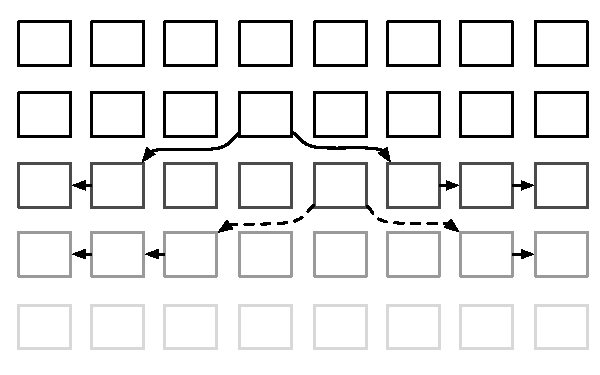
\includegraphics[width=0.4\textwidth]{figures/coordination/nqueens.pdf}
\caption{Concurrent propagation of N-Queens states.}
\label{coordination:fig:nqueens}
\end{figure}

An empty state is instantiated in the top-left square
(line~\ref{line:coord:queens_axiom}) and is then propagated to all squares in
the same row (rule in
lines~\ref{line:coord:queens_propr1}-\ref{line:coord:queens_propr2}). Once a
square $S$ receives a new state $L$, it checks if $S$ can be incorporated into
$L$. For that, it checks if there is no queen on $S$'s column (rules in lines
\ref{line:coord:queens_col1}-\ref{line:coord:queens_col2}), if there is no queen
on $S$'s left diagonal (rules in
lines~\ref{line:coord:queens_ldiag1}-\ref{line:coord:queens_ldiag2}) and if
there is no queen on $S$'s right diagonal (rules in
lines~\ref{line:coord:queens_rdiag1}-\ref{line:coord:queens_rdiag2}).

If there is any conflict, we do not derive anything and for that we use the
language expression \code{1}
(lines~\ref{line:coord:queens_empty1},~\ref{line:coord:queens_empty2}
and~\ref{line:coord:queens_emtpy3}), which corresponds to an empty rule head. If
there are no conflicts, this means that it is possible to add a queen to the
current state (line~\ref{line:coord:queens_add}). The fact \code{send-down/2} is
used to either complete the computation of a valid state
(lines~\ref{line:coord:queens_complete1}-\ref{line:coord:queens_complete2}) or
to propagate the state to the row below
(lines~\ref{line:coord:queens_down1}-\ref{line:coord:queens_down2}) as shown in
Fig.~\ref{coordination:fig:nqueens}.

Most popular parallel implementations of the N-Queens problem
distribute the search space of the problem by assigning incomplete
boards as tasks to threads. Our approach is unusual because the tasks
are the squares of the board.

\begin{figure}[h!]
\begin{Verbatim}[numbers=left,fontsize=\codesize,commandchars=\*\#\&]
type list int state.

type left(node, node).
type right(node, node).
type down-left(node, node).
type down-right(node, node).
type coord(node, int, int).
type linear propagate-left(node, state).
type linear propagate-right(node, state).
type linear test-y(node, int, state, state).
type linear test-diag-left(node, int, int, state, state).
type linear test-diag-right(node, int, int, state, state).
type linear send-down(node, state).
type linear new-state(node, state).
type linear final-state(node, state).

propagate-right(@0, []).*label#line:coord:queens_axiom&

propagate-left(A, State)
  -o {L | !left(A, L), L <> A | propagate-left(L, State)},
     new-state(A, State).
propagate-right(A, State)*label#line:coord:queens_propr1&
  -o {R | !right(A, R), R <> A | propagate-right(R, State)},
     new-state(A, State).*label#line:coord:queens_propr2&

new-state(A, State), !coord(A, X, Y)
  -o test-y(A, Y, State, State).

// check if there is no queen on the same column*label#line:coord:queens_col1&
test-y(A, Y, [], State), !coord(A, OX, OY)
  -o test-diag-left(A, OX - 1, OY - 1, State, State).
test-y(A, Y, [X, Y1 | RestState], State), Y = Y1
  -o 1. // fail*label#line:coord:queens:empty1&
test-y(A, Y, [X, Y1 | RestState], State), Y <> Y1
  -o test-y(A, Y, RestState, State).*label#line:coord:queens_col2&

// check if there is no queen on the left diagonal*label#line:coord:queens_ldiag1&
test-diag-left(A, X, Y, _, State), X < 0 || Y < 0, !coord(A, OX, OY)
  -o test-diag-right(A, OX - 1, OY + 1, State, State).
test-diag-left(A, X, Y, [X1, Y1 | RestState], State), X = X1, Y = Y1
  -o 1. // fail*label#line:coord:queens:empty2&
test-diag-left(A, X, Y, [X1, Y1 | RestState], State), X <> X1 || Y <> Y1
  -o test-diag-left(A, X - 1, Y - 1, RestState, State).*label#line:coord:queens_ldiag2&

// check if there is no queen on the right diagonal*label#line:coord:queens_rdiag1&
test-diag-right(A, X, Y, [], State), X < 0 || Y >= size, !coord(A, OX, OY)
  -o send-down(A, [OX, OY | State]). // add new queen*label#line:coord:queens_add&
test-diag-right(A, X, Y, [X1, Y1 | RestState], State), X = X1, Y = Y1
  -o 1. // fail*label#line:coord:queens:empty3&
test-diag-right(A, X, Y, [X1, Y1 | RestState], State), X <> X1 || Y <> Y1
  -o test-diag-right(A, X - 1, Y + 1, RestState, State).*label#line:coord:queens_rdiag2&

send-down(A, State), !coord(A, size - 1, _)*label#line:coord:queens_complete1&
  -o final-state(A, State).*label#line:coord:queens_complete2&
send-down(A, State), !coord(A, CX, _), CX <> size - 1*label#line:coord:queens_down1&
  -o {B | !down-right(A, B), B <> A | propagate-right(B, State)},
     {B | !down-left(A, B), B <> A | propagate-left(B, State)}.*label#line:coord:queens_down2&
\end{Verbatim}
  \caption{N-Queens problem solved in LM.}
  \label{coordination:code:nqueens}
\end{figure}

\subsubsection{Proof Of Correctness}

\begin{lemma}[test-y lemma]

If \code{test-y(A, Y, State, OriginalState)} then either $\exists_{x'}. {(x',
y) \in \mathtt{State}}$ and \code{test-y} is consumed or
\code{test-diag-left(A, OX - 1, OY - 1, OriginalState, OriginalState)}, where
\code{OX} and \code{OY} are the coordinates of the square.

\end{lemma}
\begin{proof}
Induction on the size of \code{State}.

First rule: immediately the second conclusion.

Second rule: immediately the third conclusion.

Third rule: by induction.
\end{proof}

\begin{lemma}[test-diag-left lemma]
If \code{test-diag-left(A, X, Y, State, OriginalState)} then either $\exists_{x', y'}. {(x', y') \in \mathtt{State}}$, where $x = x' - a$ and $y' = y - a$, where $a$ is positive or $0$ and \code{test-diag-left} is consumed or \code{test-diag-right(A, OX - 1, OY + 1, OriginalState, OriginalState)}, where \code{OX} and \code{OY} are the coordinates of the square.
\end{lemma}
\begin{proof}
Induction on the size of \code{State}.

First rule: immediately the second conclusion.

Second rule: immediately the first conclusion.

Third rule: by induction.
\end{proof}

\begin{lemma}[test-diag-right lemma]
If \code{test-diag-right(A, X, Y, State, OriginalState)} then either $\exists_{x', y'}. {(x', y') \in \mathtt{State}}$, where $x = x' - a$ and $y' = y + a$, where $a$ is positive or $0$ and \code{test-diag-right} is consumed or \code{send-down(A, [(OX, OY) | OriginalState])}, where \code{OX} and \code{OY} are the coordinates of the square.
\end{lemma}
\begin{proof}
Induction on the size of \code{State}.

First rule: immediately the second conclusion.

Second rule: immediately the first conclusion.

Third rule: by induction.
\end{proof}

\begin{theorem}[State validation]
If \code{test-y(A, OY, State, State)} then either everything is consumed or \code{send-down(A, [(OX, OY) | State])} is derived, where \code{OX} and \code{OY} are the coordinates of the square and are a valid addition to the \code{State}.
\end{theorem}
\begin{proof}
Use the previous three lemmas.
\end{proof}

\begin{lemma}[Propagate left lemma]
If \code{propagate-left(A, State)} then every cell to the left, including \code{A} will derive \code{new-state(A, State)}.
\end{lemma}
\begin{proof}
By induction on the number of cells to the left of \code{A}. The only rule that uses \code{propagate-left/2} will prove the lemma.
\end{proof}

\begin{lemma}[Propagate right lemma]
If \code{propagate-right(A, State)} then every cell to the right, including \code{A} will derive \code{new-state(A, State)}.
\end{lemma}
\begin{proof}
By induction on the number of cells to the right of \code{A}. The only rule that uses \code{propagate-right/2} will prove the lemma.
\end{proof}

\begin{theorem}[States theorem]
For a given row, we will compute several \code{send-down(A, State)} facts that represent valid configurations that include that row and the rows above.
\end{theorem}
\begin{proof}
By induction on the number of rows.

For row 0, we use the axiom \code{propagate-right(@0, [])}, that will be propagated to all nodes in row 0. By using the state validation theorem, we know that every node will derive \code{send-down(A, [(X, Y)])}, all valid configurations.


By induction, we know that row $X'$ has derived every \code{send-down/2} possible. Such facts will be sent downwards to row $X = X' + 1$ using the last rule in the program, deriving \code{propagate-right} or \code{propagate-left} that will derive \code{new-state} at each right or left cell. We do not derive anything at the cell below or the ones to the sides since they would not be valid. Using the \code{new-state} fact, we get a \code{test-y} fact that will be checked using the state validation theorem, filtering all new valid configurations and deriving \code{send-down/2}.
\end{proof}

\subsection{Heat Transfer}


